\section{Der Level-Editor} \label{leveleditor}
Die Erstellung eines Levels ist in jedem Spiel sehr von Bedeutung. Dieses kann in Unity erstellt werden, indem programmiertechnisch in Skripten \textit{Prefabs} manuell instanziiert werden. Die Aufgabe der Erstellung von vielen verschiedenen Leveln wird in Unternehmen allerdings oftmals an Personen ohne tiefgreifende Kenntnisse in der Informatik weitergegeben und würde auf diese Weise zu viel Zeit in Anspruch nehmen. Um dem Spieler möglichst viel Inhalt mit möglichst geringem Entwicklungsaufwand bieten zu können, muss es möglich sein verschiedene Level leicht zu implementieren und diese testen zu können. Hierfür wird entweder ein Level-Editor oder ein Level-Generator benötigt. Das Erstellen eines Levels soll auch für Benutzer ohne Informatik-Kenntnisse geeignet sein, da diese es oft sind, die durch das Erstellen und Hinzufügen von weiteren Leveln das Interesse an diesem Spiel für die Gemeinschaft der Spieler bewahren. Um dies zu ermöglichen, wird ein Level-Editor mit grafischer Benutzeroberfläche benötigt. Im Folgenden werden Möglichkeiten zum Design eines Level-Editors untersucht. 

\subsection{Designmöglichkeiten}
Für Unity gibt es viele Tutorials, die zeigen wie man einen Level-Editor erstellt. Dabei wird meist eine sehr einfache Variante vorgestellt. Hierbei wird mit Hilfe einer Bildbearbeitungssoftware zunächst eine Karte mit Verwendung von unterschiedlichen Farben und transparentem Hintergrund erstellt wie Bild \ref{leveleditor_designarts_levelcreation} zeigt. Im Anschluss wird dieses Bild in Unity geladen und jeder farbige Pixel als ein bestimmtes Objekt interpretiert wie in Bild \ref{leveleditor_designarts_gameplay} dargestellt.

\begin{figure}[h]
    \begin{minipage}[t]{0.49\textwidth}
         \subfloat[Die Levelerstellung]{ \label{leveleditor_designarts_levelcreation}
        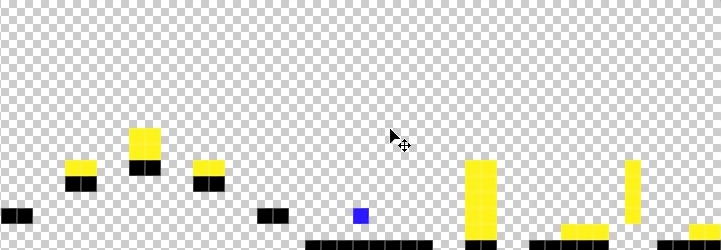
\includegraphics[width=1\textwidth]{pics/leveleditor_designarts_levelcreation.png}}
    \end{minipage}
    \hfill
    \begin{minipage}[t]{0.49\textwidth}
         \subfloat[Das erstellte Level im Spielmodus]{ \label{leveleditor_designarts_gameplay}
        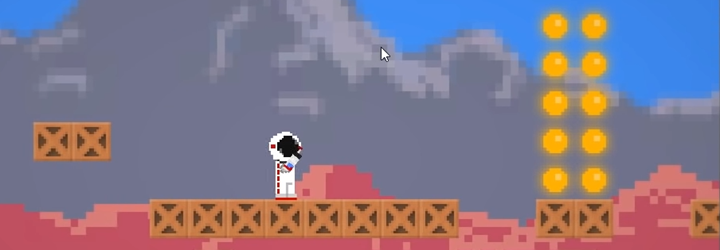
\includegraphics[width=1\textwidth]{pics/leveleditor_designarts_gameplay.png}}
    \end{minipage}
    \caption[Ein in Unity oft implementierter Level-Editor]{Ein in Unity oft implementierter Level-Editor\cite{Brackeys.2017}}
\end{figure} 

In diesem Beispiel wurde für jeden gelben Pixel eine Goldmünze zum einsammeln, für jeden schwarzen Pixel ein Flurstück zum gehen und für einen blauen Pixel die Spielerstartposition gewählt. Diese Möglichkeit des Level-Editors schaut zunächst verblüffend einfach und für jedes 2D-Spiel geeignet aus. Jedoch hat dieser Ansatz einen sehr großen Nachteil:

Für jeden möglichen Zustand eines Objektes muss prinzipiell eine eigene Farbe definiert werden. Dies bedeutet, dass alleine eine beliebig einstellbare Magazingröße einer Waffe theoretisch unendlich viele Farben zur Folge hat. Indem man die Anzahl der möglichen instanziierbaren Zustände eines Objektes beschränkt kann man diesem Problem etwas entgegenwirken. Begrenzt man die Anzahl der einstellbaren Magazingrößen auf drei verschiedene Größen für jede Waffe so erhält man für 10 Waffen 30 unterschiedliche Farben. Berücksichtigt man dabei, dass ein Feind jede beliebige Waffe oder keine tragen kann, so müssen bereits bei 3 Gegnern und dem Spieler (4 * (30 + 1)) = 124 verschiedene Farben definiert werden. Aus diesen Überlegungen ist bereits erkennbar, dass die Anzahl der zu definierenden Farben bei einer Erweiterung des Spiels sehr stark anwächst. Bereits bei über 100 verschiedenen Farben verliert ein Benutzer schnell die Übersicht. Dieses Problem wird noch verstärkt, wenn berücksichtigt werden muss, dass sich Objekte auch überlappen können. Aufgrund dieser extrem schlechten Erweiterbarkeit und Benutzerunfreundlichkeit bei größeren Spielen wurde diese Variante nicht implementiert.

%-- Unity Erweitung für Entwickler-LevelEditor: Erklärung, Begründung, wieso diese Variante nicht hergenommen wurde (alpha-Stand, Editor ist nur für Entwickler gedacht)  Eine andere Möglichkeit eines Leveleditors wird in der neuesten Version von Unity angeboten. Bei dieser Variante kann im Unity-Editor können Objekte zu einem neuen Panel eingestellt werden. Im Anschluss können diese Objekte ausgewählt und in einer Szene platziert werden. 

In Unity gibt im \textit{Asset Store} ebenfalls bereits fertige Level-Editoren zu finden. Der \textit{Asset Store} ist eine von Unity bereitgestellte Plattform, auf dem Entwickler \texttt{Assets} für andere Entwickler zur Verwendung im Spiel anbieten. \textit{Assets} können \textit{Prefabs}, aber auch Sammlungen von unterschiedlichen Arten von \textit{Prefabs} oder sogar in Unity integrierbare Softwarekomponenten wie Level-Editoren sein. Diese Editoren sind jedoch nur sehr schlecht für das bereits existierende Spiel geeignet, da bei diesen oftmals bereits Spielobjekte enthalten sind, die optisch nicht zum Spiel passen und ein großer Umbau dieser Level-Editoren stattfinden muss, um diese für das Spiel nutzen zu können. Hierzu sind Level-Editoren meist nur für Entwickler gedacht, da ein Spieler diese im Spiel nicht nutzen kann.

Dem entgegengesetzt wurde bei dem Design für den Level-Editor ein Editor zur Nutzung für Entwickler als auch Benutzer entwickelt. Ziel ist es, dass nicht nur ein Entwickler, sondern auch jeder Benutzer des Spiels die Möglichkeit haben soll, ein eigenes Level zu erstellen. Dies erlaubt eine viel größere Vielfalt an Leveln, erhöht die Menge des Spielinhalts für einen Benutzer und verringert gleichzeitig den Entwicklungsaufwand zum Erstellen von neuen herausfordernden Leveln. Dabei wurden zunächst folgende Anforderungen für den Level-Editor definiert:

\begin{enumerate}
	\item \textbf{Effizienz:} Dem Benutzer muss es möglich sein schnellstmöglich ein spielbares Level zu erstellen oder zu bearbeiten.
	\item \textbf{Benutzerfreundlichkeit:} Der Benutzer muss  komfortabel und intuitiv ohne Anleitung sofort ein Level erstellen können.
	\item \textbf{Erweiterbarkeit:} Es soll mit geringen Aufwand möglich sein bereits in das Spiel implementierte Elemente wie neue Waffen in den Level-Editor zu integrieren.
	\item \textbf{Geringe Abhängigkeiten}: Der Level-Editor stellt einen eigenen Bereich des Spiels dar. Änderungen an dem Level-Editor (und umgekehrt), mit Ausnahme der Änderung an Schnittstellen zu gemeinsamen Komponenten, sollen den jeweils anderen Bereich der Software nicht beeinträchtigen.
\end{enumerate}

Diese Anforderungen stellen sicher, dass der Benutzer gut mit dem Level-Editor arbeiten kann und somit die Bereitschaft erhöhen neue Level zu erstellen und diese mit der Gemeinschaft der Spieler und Entwickler zu teilen. Anforderung 3 stellt sicher, dass ein Entwickler kaum Aufwand betreiben muss, um ein neues Element für den Level-Editor benutzbar zu machen. Mit der letzten Anforderung soll bewirkt werden, dass Änderungen an einer Komponente die Funktionalität der jeweils anderen nicht beeinträchtigen.

\subsection{Die Benutzeroberfläche}\label{sec:user_interface}
Für die Implementierung musste ein Weg gefunden werden, um all diese Anforderungen umzusetzen. Dabei wurden zunächst Eigenschaften des Level-Editors definiert, die dem Benutzer es ermöglichen sollen besonders effizient und intuitiv ein Level zu erstellen oder zu bearbeiten. Folgende Eigenschaften wurden zur Kontrolle der Einhaltung der Anforderungen definiert:

\begin{itemize}
	\item Der Benutzer soll eine Rückmeldung erhalten, welches Objekt er bei Mausklick editieren kann.
	\item Der Benutzer soll ein Objekt per Mausklick verschieben können. Dabei soll ihm vorher angezeigt werden, welches Objekt er aktuell verschieben würde.
	\item Der Benutzer soll mit Hilfe des Verschiebens einer Waffe einen Gegner oder Spieler mit dieser bewaffnen können.
	\item Der Benutzer soll per Klick auf eine Schaltfläche, das auf der Schaltfläche angegebene Spielobjekt bei der Maus angezeigt bekommen und bei jedem Mausklick auf der Karte bei der gewählten Position eine Instanz des dort angezeigten Spielobjektes erstellen können.
	\item Mit einem Mausklick auf ein bereits platziertes Objekt sollen änderbare Eigenschaften wie Munitionsmenge bei Waffen angezeigt und durch den Benutzer leicht verändert werden können.
	\item Für Levelelemente wie Wände soll es möglich sein bei gedrückter Maustaste und gleichzeitigem Bewegen der Maus bei den Positionen des Mauszeigers automatisch Spielobjekte des ausgewählten Typs zu platzieren.
	\item Ein auf die Karte gesetztes Objekt soll ohne Änderung direkt bei Speicherung des Levels im zugehörigen Spiel verwendet werden können.
	\item Es soll möglich sein komfortabel mit der Kamera hinein- und herauszuzoomen, als auch die Position der Kamera zu ändern.
\end{itemize}

Die Interaktion des Benutzers mit dem Level-Editor geschieht durch die Benutzeroberfläche des Editors, die im Folgenden vorgestellt wird. Mit ihr und der damit verbundenen Anwendungslogik werden diese Eigenschaften erfüllt. 

\subsubsection{Die Benutzeroberfläche}
\begin {figure}[h]
	\begin {center}
	    \includegraphics[width=1\textwidth]{pics/leveleditor_interface.png}
		\caption{Die Benutzeroberfläche des Level-Editors}
		\label{fig:userinterface_leveleditor}
	\end {center}
\end {figure}

Abbildung \ref{fig:userinterface_leveleditor} zeigt die Benutzeroberfläche des Level-Editors. Diese ist unterteilt in den Le\-vel\-ver\-wal\-tungs-Bereich (links oben), den Objekterstellungs- und Lösch-Bereich (links am Rand) und den Objektbearbeitungs-Bereich (rechter Rand). 

Mit dem Levelverwaltungsbereich kann ein neues Level erstellt, ein Level geladen oder gespeichert werden. Zum Erstellen eines neuen Levels können die Textfelder \glqq{}W\grqq{} für Weite und \glqq{}H\grqq{} für Höhe genutzt werden, um die Größe des neuen Levels festzulegen und mit der Schaltfläche \glqq{}New Level\grqq{} wird dieses erstellt. Das aktuell im Editor vorhandene Level mit allen Spielobjekten wird dabei ohne Sicherung gelöscht und durch das neue Level ersetzt. Sollen die Änderungen behalten werden, so ist es wichtig das Level vorher zu speichern, um dieses mit Hilfe der gespeicherten Datei wieder in den Editor laden zu können.

Mit dem Objekterstellungs- und Lösch-Bereich können neue Spielobjekte erstellt oder bereits im Level vorhandene Objekte gelöscht werden. Hierfür muss die Schaltfläche für das zugehörige Objekt gedrückt und das ausgewählte Objekt mit der Maus auf die gewünschte Position auf der Karte mit einem Mausklick gesetzt werden. Möchte man ein Objekt löschen, so muss analog die Schaltfläche \glqq{}Deletion Mode\grqq{} gedrückt und auf das zu löschende Objekt auf der Karte mit der linken Maustaste geklickt werden.

Im Objektbearbeitungs-Bereich können Eigenschaften von Objekten bearbeitet werden. Letzterer wird sichtbar, wenn im Level-Editor auf ein markiertes Objekt geklickt wird und der Lösch- oder Platzierungsmodus nicht aktiviert ist. Hier werden für jedes Objekt spezifische Eigenschaften zum Einstellen angezeigt. Beispielsweise ist es möglich für einen Gegner eine Patroullienroute zu erstellen oder die Munitionsmenge für eine bestimmte Waffe festzulegen. Im Bild \ref{fig:userinterface_leveleditor} ist letzteres sichtbar. 

Es ist zu erwähnen, dass jedes Level bei Erstellung eine Wandumrandung an den Kanten des Levels erhält, die nicht gelöscht oder verschoben werden können. Dies wurde festgelegt, da ein Spieler oder andere Spielobjekte sich nicht über den Rand der Karte hinaus bewegen sollen.

Die Interaktion des Benutzers mit dem Level-Editor funktioniert mit Hilfe der beiden Maustasten, dem Bewegen der Maus und dem Mausrad. mit dem Mausrad kann aus der Karte hinein- und herausgezoomt werden. Wird die rechte Maustaste nur kurz gedrückt, so wechselt der Editor in den sogenannten \glqq{}Leermodus\grqq{}. Dies bedeutet der Editor verlässt den aktuellen Zustand und wechselt in den Startzustand, bei dem Objekte nicht verändert, platziert oder gelöscht werden können. Wird die rechte Maustaste gedrückt gehalten und die Maus bewegt, so kann zu einem anderen Ort der Karte mit der Kamera navigiert werden. Die linke Maustaste hat je nach Zustand eine andere Bedeutung:

\begin{itemize}
	\item \textbf{Leermodus:} 	
	\begin {itemize}
	\item Tastendruck ein markiertes Objekt: Wechsel in den Editiermodus
	\item Tastendruck auf eine freie Fläche der Karte: Keine Wirkung
	\item Auf ein markiertes Objekt wird geklickt, gehalten und die Maus bewegt: Die Position des Spielobjektes auf der Karte wird verändert
	\end{itemize}
	\item \textbf{Platzierungsmodus:} 
	\begin{itemize}
	\item Tastendruck auf ein Stück der Karte ohne Level-Element: ein neues Spielobjekt wird an der Position des Mauszeigers platziert.
	Tastendruck auf ein Stück der Karte mit Level-Element: Keine Wirkung
	\item Gedrückt halten: Ist das ausgewählte Spielobjekt ein Level-Element, so werden, wenn möglich, an den Positionen des Mauszeigers Instanzen des ausgewählten Spielobjektes erstellt.
	\end{itemize} 
	\item \textbf{Editiermodus:} 
	\begin{itemize}
	\item Tastendruck auf ein Spielobjekt: Aktualisierung des Objektbearbeitungsbereiches für das ausgewählte Spielobjekt
	\item Tastendruck auf einen leeren Fleck der Karte: Wechsel in den Leermodus und Verbergen des Objektbearbeitungsbereiches
	\end{itemize} 
	\item \textbf{Löschmodus}: 
	\begin{itemize}
	\item Tastendruck auf ein markiertes Objekt: Löschen des Objektes
	\item Gedrückt halten: Jedes Spielobjekt das markiert wird, wird sofort gelöscht.
	\end{itemize}
	\item \textbf{Modus zum Setzen von Patroullienrouten}: 
	\begin{itemize}
	\item Tastendruck Auf ein Stück der Karte ohne Level-Element: Setzen eines Wegpunktes
	\item Tastendruck Auf ein Stück der Karte mit Level-Element: Keine Wirkung
	\end{itemize}  
\end{itemize}

Wird im Modus für das Setzen der Patroullienroute eines Gegners dieser Modus verlassen, so wird die für den Gegner bis dahin gesetzte Patroullienroute gespeichert. Das Arbeiten mit diesen Zuständen soll die Steuerung des Level-Editors für den Benutzer erleichtern, da ansonsten unnötig viele Tasten für unterschiedliche Funktionalität belegt werden müssten. Für Details zur Umsetzung des Level-Editors wird auf die im nachfolgenden Abschnitt vorgestellte Implementierung verwiesen.

%Mit Hilfe des Levelverwaltungs-Bereiches kann ein neues Level mit einer beliebigen Größe erstellt, ein bereits existierendes Level zum Editieren geladen oder ein bereits erstelltes Level gespeichert werden.

%Beim Drücken der Schaltfläche "Neues Level" werden die in den Textfeldern vorhandenen Werte ausgelesen und die Funktion CreateLevel(...) des LevelCreators übergeben. 


%Bei Klick auf einer dieser Schaltflächen wird das Flag für den Platzierungsmodus gesetzt und eine Instanz des ausgewählten Prefabs erstellt welches der Maus folgt. Bei einem Mausklick auf die Karte wird dort wo sich das der Maus folgende SpielObjekt befindet ein weiteres Objekt dieser Art instanziiert, in das Verzeichnis für die auf der Karte befindlichen Spielobjekte eingetragen (inScenePlacedObjects). Da sich Levelelemente und Objekte anderen Typs nicht gleichzeitig auf einem Kartenstück befinden können, wird hinterlegt auf welchem Kartenstück sich das Spielobjekt befindet.


%Wird die Schaltfläche für das Laden eines Levels gedrückt, so ruft der InterfaceButtonHandler die Funktion LoadLevel() des LevelCreators auf, welcher den Befehl zum Laden der Daten an den LevelController mit Hilfe der Funktion LoadLevelData() übergibt und danach die Daten mit Hilfe des LevelDatenManagers mit Hilfe der Funktion GetLevelData() abruft und dem Modul LevelPlacement über die Funktion PlaceObjects(...) die SpielObjekte für das Level erstellen und platzieren lässt.    

%Wird die Schaltfläche zum Speichern des Levels gedrückt, so ruft der InterfaceButtonHandler die Funktion SaveLevel() des LevelCreators auf, welche die auf der Karte platzierten Objekte dem LevelDataManager mit Hilfe der Funktion SaveLevelData(...) zum Speichern übergibt und nach der Speicherung der Objekte dem LevelController den Befehl zur Serialisierung der Spielobjekte mit Hilfe der Funktion SaveLevel() übergibt. 

%Wird auf ein Objekt mit der Maus geklickt ohne im Lösch- oder Platzierungsmodus zu sein wird das Flag für den Editiermodus gesetzt. Wird auf ein anderes Objekt geklickt so wird das neu ausgewählte Objekt bearbeitet. Wird hingegen auf kein Objekt geklickt, so wird der Editiermodus verlassen und es wird weder ein Objekt erstellt, gelöscht oder bearbeitet. Wird ein Gegner ausgewählt so können die Wegpunkte für diesen Gegner gesetzt werden. Hierfür muss im zu dem zugehörigen Objekteditorfenster in der Benutzeroberfläche die Schaltfläche "Start" zum Starten des WegPlatzierungsmodus gedrückt werden. Wird dieser gedrückt, so können über einen Klick auf die Karte die Wegpunkte nacheinander für den Gegner gesetzt werden. Wird auf die Schaltfläche "Stop" gedrückt oder einer der anderen Modusse über das Drücken der jeweiligen Schaltfläche gestartet, so wird werden die aktuell gesetzten Wegpunkte in dem Gegner-Spielobjekt gespeichert. 

%Im Objektbearbeitungsbereich können Levelelemente, Gegner und Waffen erzeugt, gelöscht oder bearbeitet werden. Im InterfaceManager sind diese in die zwei Benutzerbereiche Objektbearbeitung und Objekterstellung/-löschung unterteilt. Abbildung \ref{fig:object_management} zeigt den dazugehörigen internen Aufbau. Aus Gründen der Übersichtlichkeit wurden im LevelCreator Abhängigkeiten zu anderen Komponenten und Attribute in der Klasse PlacedObject weggelassen, die aus dem zugehörigen Interface ersichtlich sind. 

\subsection{Die Implementierung}\label{sec:implementation}
\begin {figure}[h]
	\begin {center}
	    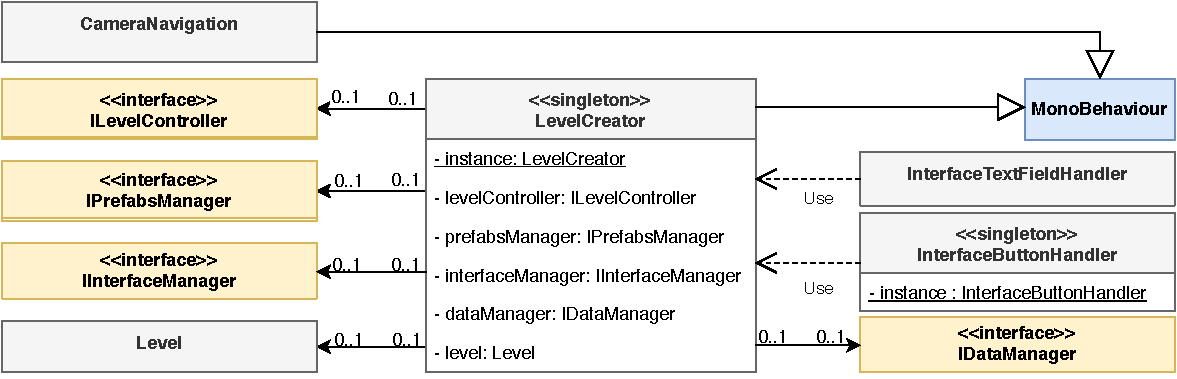
\includegraphics[width=1\textwidth]{pics/leveleditor_core.pdf}
		\caption{Der Level-Editor mit seinen Kernkomponenten}
		\label{fig:leveleditor_core}
	\end {center}
\end {figure}

Der Level-Editor stellt einen eigenständigen Bereich des Spiels dar. Für die Umsetzung des Editors konnten folgende Aufgabenbereiche identifiziert werden:

\begin{itemize}
	\item Die Ereignisbehandlung: Die Kommunikation der Komponenten bei Benutzeraktionen
	\item Die Kameranavigation
	\item Die Verwaltung der \textit{Prefabs}	
	\item Die Verwaltung und Aktualisierung der Benutzeroberfläche
	\item Die Datenverwaltung
	\item Das Platzieren, Löschen und Editieren von Spielobjekten
	\item Das Laden und Speichern eines Levels
\end{itemize} 

Für jeden dieser Aufgabenbereiche wurde eine eigenständige Komponente entwickelt. Abbildung \ref{fig:leveleditor_core} zeigt die Abhängigkeiten der Kernkomponente \texttt{LevelCreator} zu den anderen intern verwendeten Komponenten. Dieses \textit{UML}-Diagramm soll einen Überblick über die Kernkomponenten des Level-Editors geben. Hierfür wurden die Methoden der zu den Komponenten gehörigen Interfaces und Klassen weggelassen. Der \texttt{LevelCreator} stellt die zentrale Komponente dar, die zusätzlich zu seiner eigenen Funktionalität sich auch um die Weiterleitung von Informationen an die anderen Komponenten kümmert. Um ein sogenanntes Gottobjekt, ein Objekt das alles weiß, zu vermeiden wurde für jeden Aufgabenbereich eine eigenständige Komponente entwickelt und jeder dieser Komponenten wird ausschließlich über die in der Abbildung dargestellten Schnittstellen nach dem \textit{Facade}-Entwurfsmuster\cite{Gamma.2011} angesprochen. Tabelle \ref{table:task_component_association} zeigt die Zuordnung der Aufgabengebiete zu den Komponenten.

\begin{table}[h]
\begin {tabularx}{\linewidth}{
    | >{\hsize=1.0\hsize}X| % 50% of 2\hsize 
    >{\hsize=1.0\hsize}X|% 50% of 2\hsize 
       % sum=2.0\hsize for 2 columns
  }
  \hline
  	    \textbf{Aufgabengebiet} & \textbf{Komponente} \\ [1.0ex]
		\hline
		 Die Ereignisbehandlung & \texttt{InterfaceButtonHandler/ TextFieldHandler} \\[0.5ex]
		 \hline
		 Die Kameranavigation & \texttt{CameraNavigation} \\[0.5ex]
		 \hline
		Die Verwaltung der \textit{Prefabs} & \texttt{PerfabsManager} \\[0.5ex] \hline
		 Die Verwaltung und Aktualisierung der Benutzeroberfläche & \texttt{InterfaceManager} \\[0.5ex]
		 \hline
		 Die Datenverwaltung & \texttt{DataManager} \\[0.5ex]
		 \hline
		Das Platzieren, Löschen und Editieren von Spielobjekten & \texttt{LevelCreator} \\[0.5ex]
		\hline
		Laden und Speichern eines Levels & \texttt{LevelController} \\[0.5ex]
		\hline
\end{tabularx}
\caption{Die Zuordnung der Aufgabengebiete zu den verwendeten Komponenten}
\label{table:task_component_association}
\end{table}

Durch das Einführen von Interfaces zwischen diesen Komponenten, werden die Abhängigkeiten der Komponenten voneinander auf ein Minimum reduziert. Zusätzlich wurde eine Hierarchie eingeführt, um zyklische Abhängigkeiten zu verhindern. Die einzigen Komponenten die auf den \texttt{LevelCreator} zugreifen sind die Komponenten für die Ereignisbehandlung und auch nur dann, wenn der Benutzer ein Ereignis beispielsweise durch das Drücken einer Schaltfläche ausgelöst hat. Der \texttt{LevelCreator} leitet die für die anderen Kernkomponenten benötigten Informationen weiter und kümmert sich um die Koordination und Initialisierung dieser Komponenten.

Im Folgenden wird die Implementierung für die verschiedenen Komponenten vorgestellt. Dabei werden diese nach der folgenden Reihenfolge vorgestellt:

\begin{enumerate}
	\item Die Ereignisbehandlung
	\item Die Kameranavigation
	\item Der Begriff \textit{Prefab} im Level-Editor
	\item Die Verwaltung der \textit{Prefabs}	
	\item Die Verwaltung und Aktualisierung der Benutzeroberfläche
	\item Das Platzieren, Löschen und Editieren von Spielobjekten
	\item Die Datenverwaltung und das Laden und Speichern eines Levels
\end{enumerate} 

\subsubsection{Die Ereignisbehandlung: Die Kommunikation der Komponenten bei Benutzeraktionen} \label{chapter:eventmanagement}
\begin {figure}[h]
	\begin {center}
	    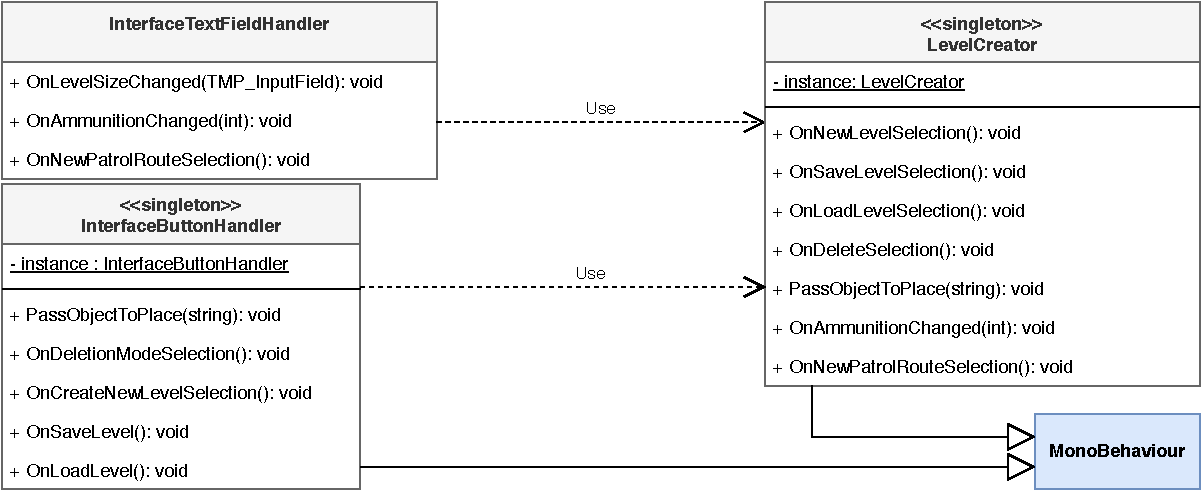
\includegraphics[width=1\textwidth]{pics/leveleditor_eventhandler.pdf}
		\caption{Die Ereignisbehandlung des Level-Editors}
		\label{fig:eventhandler}
	\end {center}
\end {figure}

Abbildung \ref{fig:eventhandler} zeigt die beteiligten Komponenten für die Ereignisbearbeitung. Es gibt zwei Komponenten, die Ereignisse abfangen: Der \texttt{InterfaceTextFieldHandler} für Ereignisse ausgelöst von Textfeldern und der \texttt{InterfaceButtonHandler} für Ereignisse ausgelöst durch das Drücken von Schaltflächen. Dabei gibt es folgende Fälle bei denen Ereignisse ausgelöst werden:

\begin{enumerate}
	\item Änderung des Textfeldes für die Weite oder Höhe eines neuen Levels
	\item \glqq{}New Level\grqq{}-Schaltfläche drücken
	\item \glqq{}Deletion Mode\grqq{}-Schaltfläche wird gedrückt
	\item Drücken einer Schaltfläche zum Platzieren eines Spielobjektes auf die Karte
	\item Änderung der Munitionsmenge im Objekt-Editor Bereich
	\item Erstellung oder Löschung einer Patroullienroute eines Spielobjektes
	\item \glqq{}Load Level\grqq{}-Schaltfläche drücken
	\item \glqq{}Save Level\grqq{}-Schaltfläche drücken
\end{enumerate}

In allen Fällen wird immer eine Funktion des \texttt{LevelCreators} aufgerufen, welcher die Bearbeitung dieser Aufgabe an andere Module übergibt und im Fall mehrerer beteiligten Komponenten sich um die schrittweisige Bearbeitung dieser Aufgabe kümmert.

Von dieser Regel gibt es nur eine einzige Ausnahme: Der erste Fall. Bei der Änderung des Textes in den Textfeldern für die Weite oder Höhe eines neuen Levels wird der \texttt{LevelCreator} und auch sonst keine andere Komponente miteinbezogen. Ein von Unity integrierter Validator kümmert sich darum, dass nur \textit{integer} Werte im zweistelligen Wertebereich eingegeben werden dürfen, während der \texttt{InterfaceTextfieldhandler} selbst überprüft, ob der neu eingegebene Wert im Wertebereich von 10 bis 99 liegt. Falls dem nicht so ist, so wird der Wert auf den Standardwert 30 gesetzt.

Beim Drücken der Schaltfläche \glqq{}New Level\grqq{} werden die in den Textfeldern vorhandenen Werte ausgelesen und der Funktion \texttt{OnNewLevelSelection(...)} des \texttt{LevelCreators} übergeben. Dieser löscht daraufhin das vorhandene Level und erstellt mit den übergebenen Werten ein Neues.

In den Fällen 3 und 4 wechselt der \texttt{Level-Editor} in den Zustand Löschmodus für das Löschen von Spielobjekten oder in den Platziermodus und zeigt das auf der Karte platzierbare Spielobjekt bei dem Mauszeiger an.

Das Erstellen oder Löschen der Patroullienroute oder die Änderung der Munitionsmenge findet im Objekteditier-Bereich der Benutzeroberfläche statt.  
Die Änderung der Munitionsmenge führt zum Aufruf der Funktion \texttt{OnAmmunitionChanged()} des \texttt{LevelCreators}, welcher die Munitionsmenge mit Hilfe eines eigenen Moduls \texttt{Objekteditier-Modul} des Objektes anpasst und dem \texttt{InterfaceManager} das aktualisierte Objekt zur Aktualisierung der Benutzeroberfläche übergibt.

Beim Aufruf der Funktion \texttt{OnNewPatrolRouteSelection()} hingegen, ausgelöst durch die Schaltfläche \glqq{}New Patrol Route\grqq{}, gibt der \texttt{LevelCreator} seinem Modul \texttt{ObjectDeletionModule} die Anweisung zum Löschen der Patroullienroute und versetzt ihn in den Modus für das Setzen einer neuen Patroullienroute. 

Die Bearbeitung der letzten beiden Fälle wird im Abschnitt \glqq{}Die Datenverwaltung und das Laden und Speichern eines Levels\grqq{} erklärt.

\subsubsection{Die Kameranavigation}
\begin {figure}[h]
	\begin {center}
	    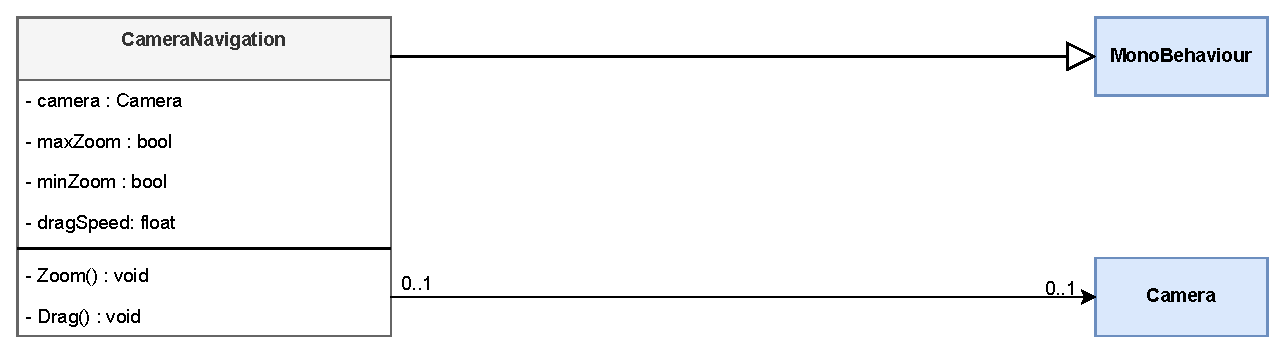
\includegraphics[width=1\textwidth]{pics/leveleditor_cameranavigation.eps}
		\caption{Die Kameranavigation im Level-Editor}
		\label{fig:leveleditor_cameranavigation}
	\end {center}
\end {figure}
Die Kameranavigation kontrolliert die Kamera des Level-Editors. Wie bereits beschrieben ist es im Level-Editor möglich über das Scrollen mit dem Mausrad zu einem Punkt der Karte hinein- und wieder herauszuzoomen. Hierfür wird intern die Funktion \texttt{Zoom()} verwendet. Desweiteren kann bei gedrückt halten der rechten Maustaste und Änderung gleichzeitigem Bewegen der Maus die Position der Kamera geändert und so ein anderer Ort der Karte bearbeitet werden. Hierfür wird die Funktion \texttt{Drag()} genutzt.


\subsubsection{Der Begriff \textit{Prefab} im Level-Editor}
\begin {figure}[h]
	\begin {center}
	    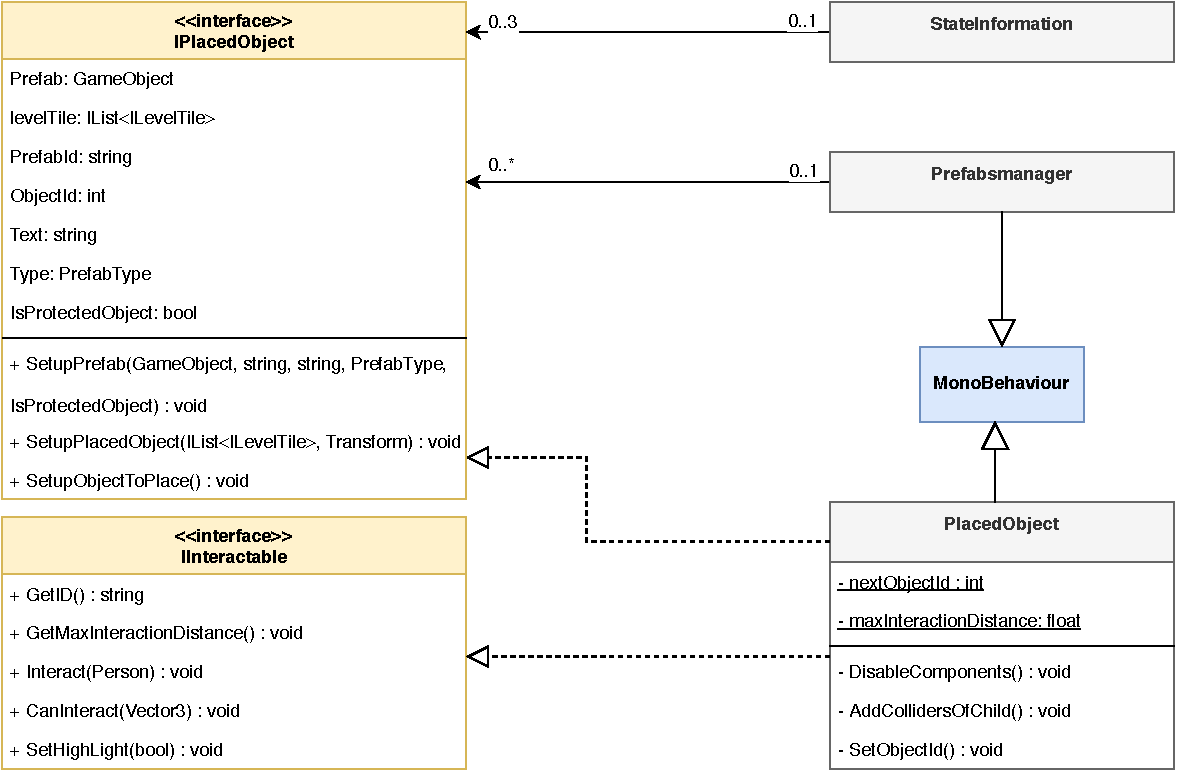
\includegraphics[width=1\textwidth]{pics/leveleditor_placedobject.pdf}
		\caption{Der Aufbau des verwendeten Containerobjekt \texttt{PlacedObject}}
		\label{fig:leveleditor_placedobject}
	\end {center}
\end {figure}

Um auf ein bestimmtes Objekt einzuwirken, ob es zu löschen, bearbeiten oder zu verschieben, ist es zunächst nötig dafür zu sorgen, dass der Benutzer weiß welches Objekt die Aktion betrifft. Hierfür kann der bereits implementierte \texttt{InteractableHoverHandler} benutzt werden. Durch diesen wird ein Objekt blau hinterlegt, wenn er mit der Maus über dieses Objekt fährt und mit Hilfe des \texttt{InteractableProximityChecker} kann auf dieses Objekt zugegriffen werden. Um diese Komponenten im Level-Editor nutzen zu können, muss jedes Objekt, das markiert werden soll das Interface \texttt{IInteractable} implementieren. Im eigentlichen Spiel soll es allerdings nicht vorkommen, dass eine Tür beispielsweise blau markiert wird oder gar verschoben werden kann. Um es trotzdem zu ermöglichen Level-Elemente wie Wände oder Türen und Gegner oder den Spieler markieren zu können, und die Abhängigkeiten des Level-Editors zum eigentlichen Spiel so gering wie möglich zu halten, wurde eine Art Container-Objekt eingeführt. Jedem Spielobjekt egal welchen Typs wurde ein Objekt übergeordnet und bestimmte Komponenten des Spielobjektes deaktiviert, da sonst beim Setzen eines Gegners und eines Spielers der Gegner den Spieler anfangen würde anzugreifen. Dadurch ist es möglich weiterhin auf die spezifischen Eigenschaften der Spielobjekte zuzugreifen, während die Interaktion auf diese Objekte über das Container-Objekt gehandhabt wird. Somit können direkte Abhängigkeiten vermieden werden, was dazu führt, dass für das Platzieren und Verwalten von Spielobjekten im Level egal ist, um welches Spielobjekt es sich genau handelt. 

Abbildung \ref{fig:leveleditor_placedobject} zeigt den internen Aufbau dieses Container-Objektes. Durch die Implementierung des Interfaces \texttt{IInteractable} und die Verlagerung des \textit{Colliders} des Spielobjektes zum Container-Objekt werden nicht mehr die durch das Interface importierten Funktionen des Spielobjektes aufgerufen, sondern die des Container-Objektes. Dadurch ist es auch mit der Methode \texttt{Interact()} möglich einem Gegner oder Spieler eine Waffe zu geben oder die Spielobjekte auf der Karte zu verschieben. Da ein \textit{Collider} nur ein Spielobjekt besitzen kann, muss das Container-Objekt von der Unity-Klasse \textit{MonoBehaviour} erben. Aus Gründen der Übersichtlichkeit wurden die aus den Interfaces importieren ersichtlichen Attribute und Methoden im Container-Objekt weggelassen. 

Das Container-Objekt hat folgende Attribute:

\begin{itemize}
	\item \textbf{objectId:} Die Objekt-Id mit der jedes platzierte Objekt eindeutig identifiziert werden kann.
	\item \textbf{Text:} Der Text der bei der zugehörigen Schaltfläche in der Benutzeroberfläche angezeigt wird.
	\item \textbf{Prefab:} Das untergeordnete Spielobjekt.
	\item \textbf{Type:} Der Typ des Spielobjektes, also ob es sich um ein Level-Element, Spieler, Gegner oder eine Waffe handelt.
	\item \textbf{LevelTile:} Auf welchem Stück oder Stücken der Karte das Spielobjekt platziert ist 
	\item \textbf{PrefabId:} Der Identifikator mit dem bei Klick auf eine Schaltfläche für das Setzen eines \textit{Prefabs} festgestellt werden kann, welches \textit{Prefab} ausgewählt wurde. Diese ID wird dem \texttt{PrefabsManager} übergeben, um eine Instanz des zugehörigen \textit{Prefabs} zu erhalten.
	\item \textbf{IsProtedObject:} Dieses Flag legt fest, ob das Objekt gelöscht oder verändert werden darf. Dies ist für die Randbegrenzung wichtig, da dort Wände nicht verschoben oder sogar gelöscht werden dürfen.
\end{itemize}

Der Typ des Spielobjektes ist unter anderem wichtig, um später entscheiden zu können, welche Eigenschaften bei dem jeweiligen Spielobjekt zum Ändern angezeigt werden. 

Dieses neue \textit{Prefab} stellt das Objekt dar, mit dem alle Komponenten des Level-Editors arbeiten. Dabei greifen alle Komponenten ausschließlich über das zugehörige Interface \texttt{IPlacedObject} auf dieses \textit{Prefab} zu. Die Komponenten, die eine Referenz auf ein solches Container-Objekt speichern sind der \texttt{LevelCreator} und der \texttt{PrefabsManager}. Der \texttt{LevelCreator} speichert in seinem Objekt \texttt{StateInformation} temporär Instanzen von \textit{Prefabs} ein, um weitere Klone von diesen Erstellen zu können oder diese zu bearbeiten. Der \texttt{PrefabsManager} hingegen verwaltet die eigentlichen \textit{Prefabs}. Dieser wird im nächsten Abschnitt genauer erläutert.

\subsubsection{Die Verwaltung der \textit{Prefabs}}
\begin {figure}[h]
	\begin {center}
	    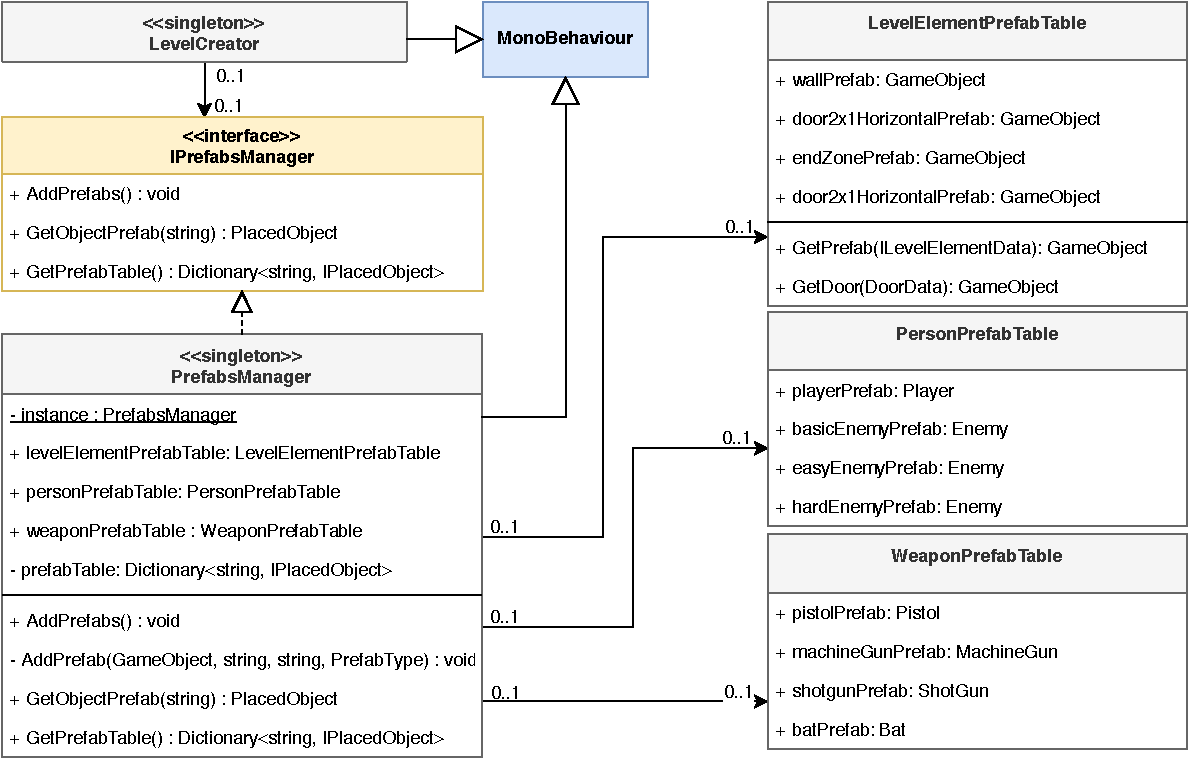
\includegraphics[width=1\textwidth]{pics/leveleditor_prefabsmanager.pdf}
		\caption{Der \texttt{PrefabsManager} des Level-Editors}
		\label{fig:prefabsmanager}
	\end {center}
\end {figure}

Wird der Level-Editor gestartet, so werden als erstes die \textit{Prefabs} für das Erstellen von neuen Spielobjekten geladen und jedes dieser \textit{Prefabs} ein Container-Objekt übergeordnet, das mit Informationen zu diesem \textit{Prefab} angereichert wird. Daraus entsteht ein neues temporär existierendes \textit{Prefab} zur Verwendung im Level-Editor. Das Klassendiagramm in Abbildung \ref{fig:prefabsmanager} gibt einen Überblick über die interne Implementierung des \texttt{PrefabsManager}. Wie zu sehen ist greift der \texttt{PrefabsManager} dabei auf die in den Tabellen \texttt{LevelElementPrefabTable}, \texttt{PersonPrefabTable} und \texttt{WeaponPrefabTable} gespeicherten \textit{Prefabs} zu. Die Funktion \texttt{Add- \linebreak Prefabs()} dient zur Initialisierung der \texttt{PrefabTabelle}. Dadurch kann der \texttt{LevelCreator} die Initialisierung der Komponenten steuern. Die Funktion \texttt{GetPrefabTable()} bewirkt schließlich, dass der \texttt{PrefabsManager} eine Kopie der intern verwendeten Tabelle zur Speicherung und Zuordnung der \textit{Prefabs} übergibt. Diese Kopie wird dem \texttt{IntefaceManager} zur Initialisierung übergeben. 

Neben dem Laden der \textit{Prefabs} kümmert der \texttt{PrefabsManager} sich auch um die Verwaltung dieser. Dabei ist es wichtig, dass die \textit{Prefabs} von Komponenten anderer Aufgabenbereiche zur Laufzeit nicht verändert werden können, da eine Änderung dieser zur Laufzeit auch eine permanente Änderung der in Unity hinterlegten \textit{Prefabs} zur Folge hätte. Daher erstellt der \texttt{PrefabsManager} auf Anfrage eines \textit{Prefabs} mit der Funktion \texttt{GetObjectPrefab(...)} eine neue Instanz des angefragten \textit{Prefabs} und übergibt diese. 

\subsubsection{Die Verwaltung und Aktualisierung der Benutzeroberfläche}

\begin {figure}[H]
	\begin {center}
	    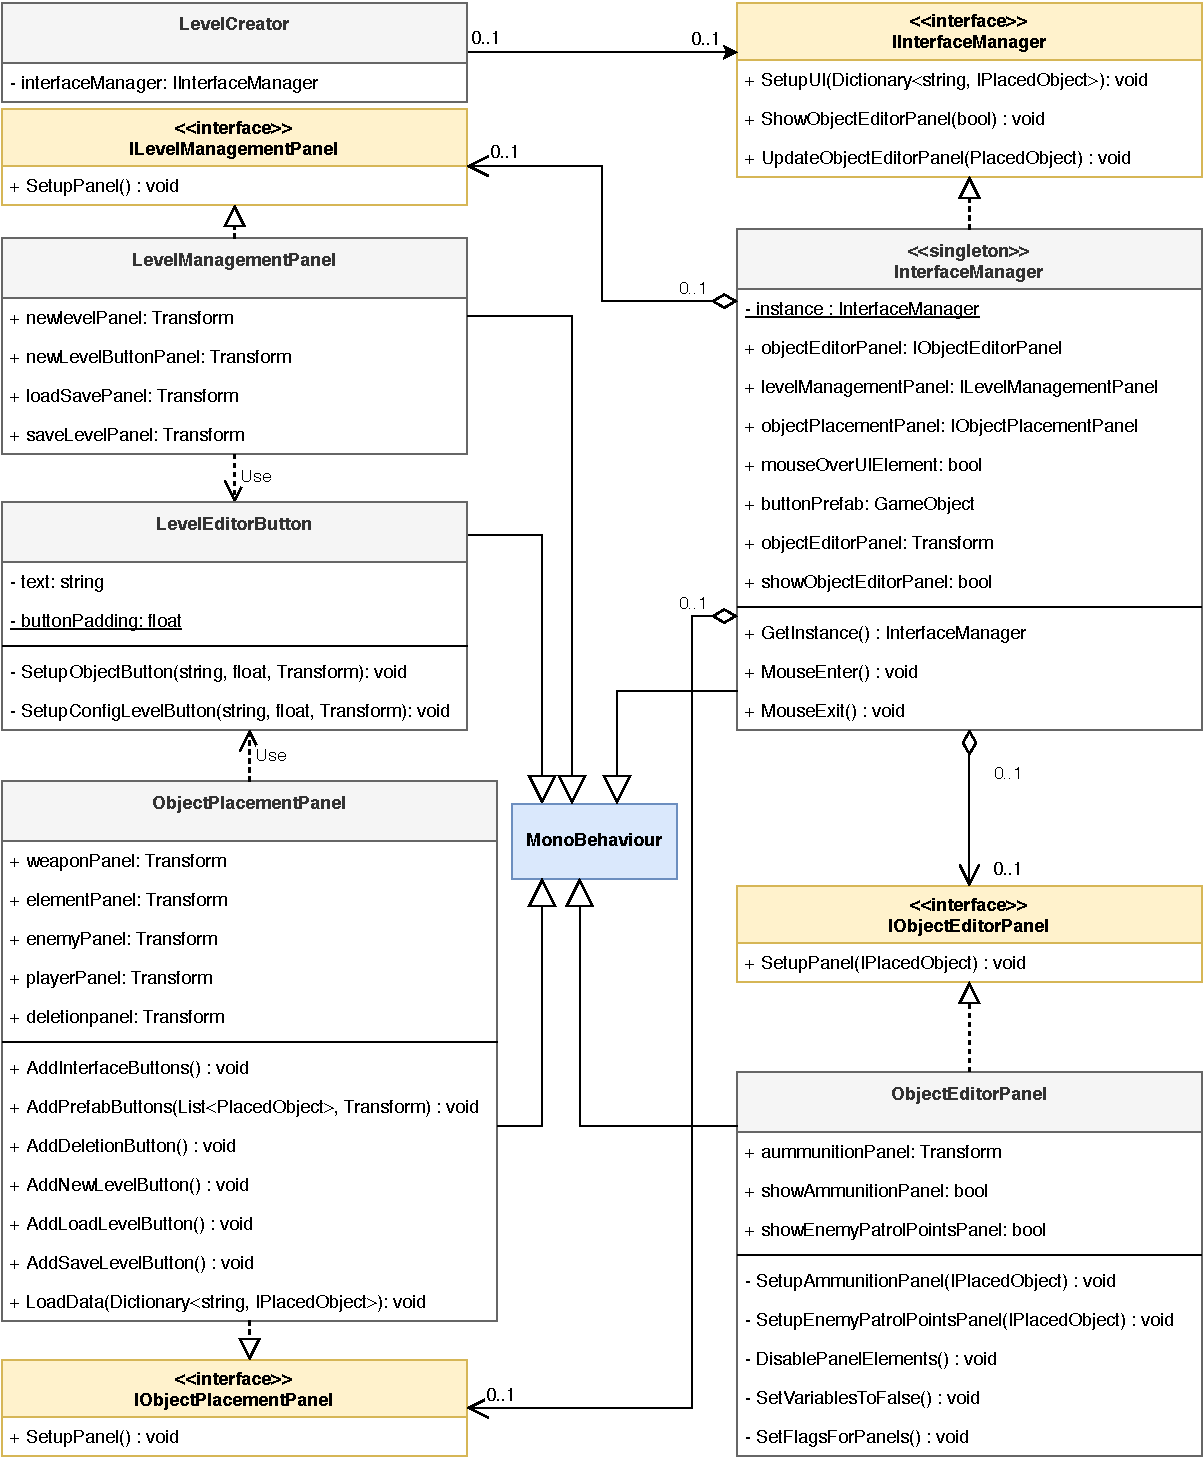
\includegraphics[width=1\textwidth]{pics/leveleditor_interfacemanager.pdf}
		\caption{Der \texttt{InterfaceManager}: Die Verwaltung der Benutzeroberfläche des Level-Editors}
		\label{fig:interfacemanager}
	\end {center}
\end {figure}

Mit Hilfe des \texttt{InterfaceManagers} wird die Benutzeroberfläche erstellt, aktualisiert und verschiedene Bereiche des Objekteditor-Bereiches der Benutzeroberfläche je nach Typ des im Editor ausgewählten \textit{Prefabs} angezeigt oder verborgen. Nach dem Laden der \textit{Prefabs} übergibt der \texttt{LevelCreator} die \textit{Prefabs}-Tabelle zum Auslesen an den \texttt{InterfaceManager}, um die Schaltflächen für alle platzierbaren Spielobjekte im Objekterstellungs- und Lösch-Bereich für die Benutzeroberfläche einzurichten. Dadurch kann bei Mausklick auf eine Schaltfläche später die hinterlegte ID des \textit{Prefabs} an den \texttt{PrefabsManager} übergeben werden, welcher eine neue Instanz des \textit{Prefabs} zum Platzieren übergibt. Abbildung \ref{fig:interfacemanager} zeigt die interne Implementierung des \texttt{InterfaceManagers}. Dieser ist intern in vier Bereiche unterteilt: Der \texttt{InterfaceManager} zur Gesamtverwaltung der Benutzeroberfläche und drei weitere eigenständige Komponenten für die im Kapitel Benutzeroberfläche vorgestellten Bereiche. 

Für die Interaktion des \texttt{LevelCreators} mit dem \texttt{InterfaceManager} werden die Funktionen \texttt{SetupUI(...)} zur Initialisierung der Benutzeroberfläche, die Funktion \texttt{ShowObjectEditor- \linebreak Panel(...)} zur Anzeige des Objekteditor-Bereiches, wenn sich der Editor im Zustand der Objektbearbeitung befindet, und die zugehörige Funktion \texttt{UpdateObjectEditorPanel(...)}. Mit dieser Funktion wird das auf der Karte ausgewählte Objekt übergeben und somit dem \texttt{InterfaceManager} alle Informationen zur Aktualisierung des Objekteditor-Bereiches übergeben. Für die Aktualisierung dieses Bereiches kümmert sich die Teilkomponente \texttt{ObjectEditorPanel}, an dem das dem \texttt{InterfaceManager} übergebene Objekt weitergereicht wird. Bei jeder Änderung der Textfelder, wird dieser Komponente das neue veränderte Objekt übergeben und aktualisiert den Objektbearbeitungs-Bereich. Die beiden anderen Bereiche, die Levelverwaltung und Objekterstellung und -löschung müssen nicht aktualisiert werden, da diese keine Felder zur Änderung des Zustandes eines Spielobjektes besitzen.

\begin {figure}[H]
	\begin {center}
	    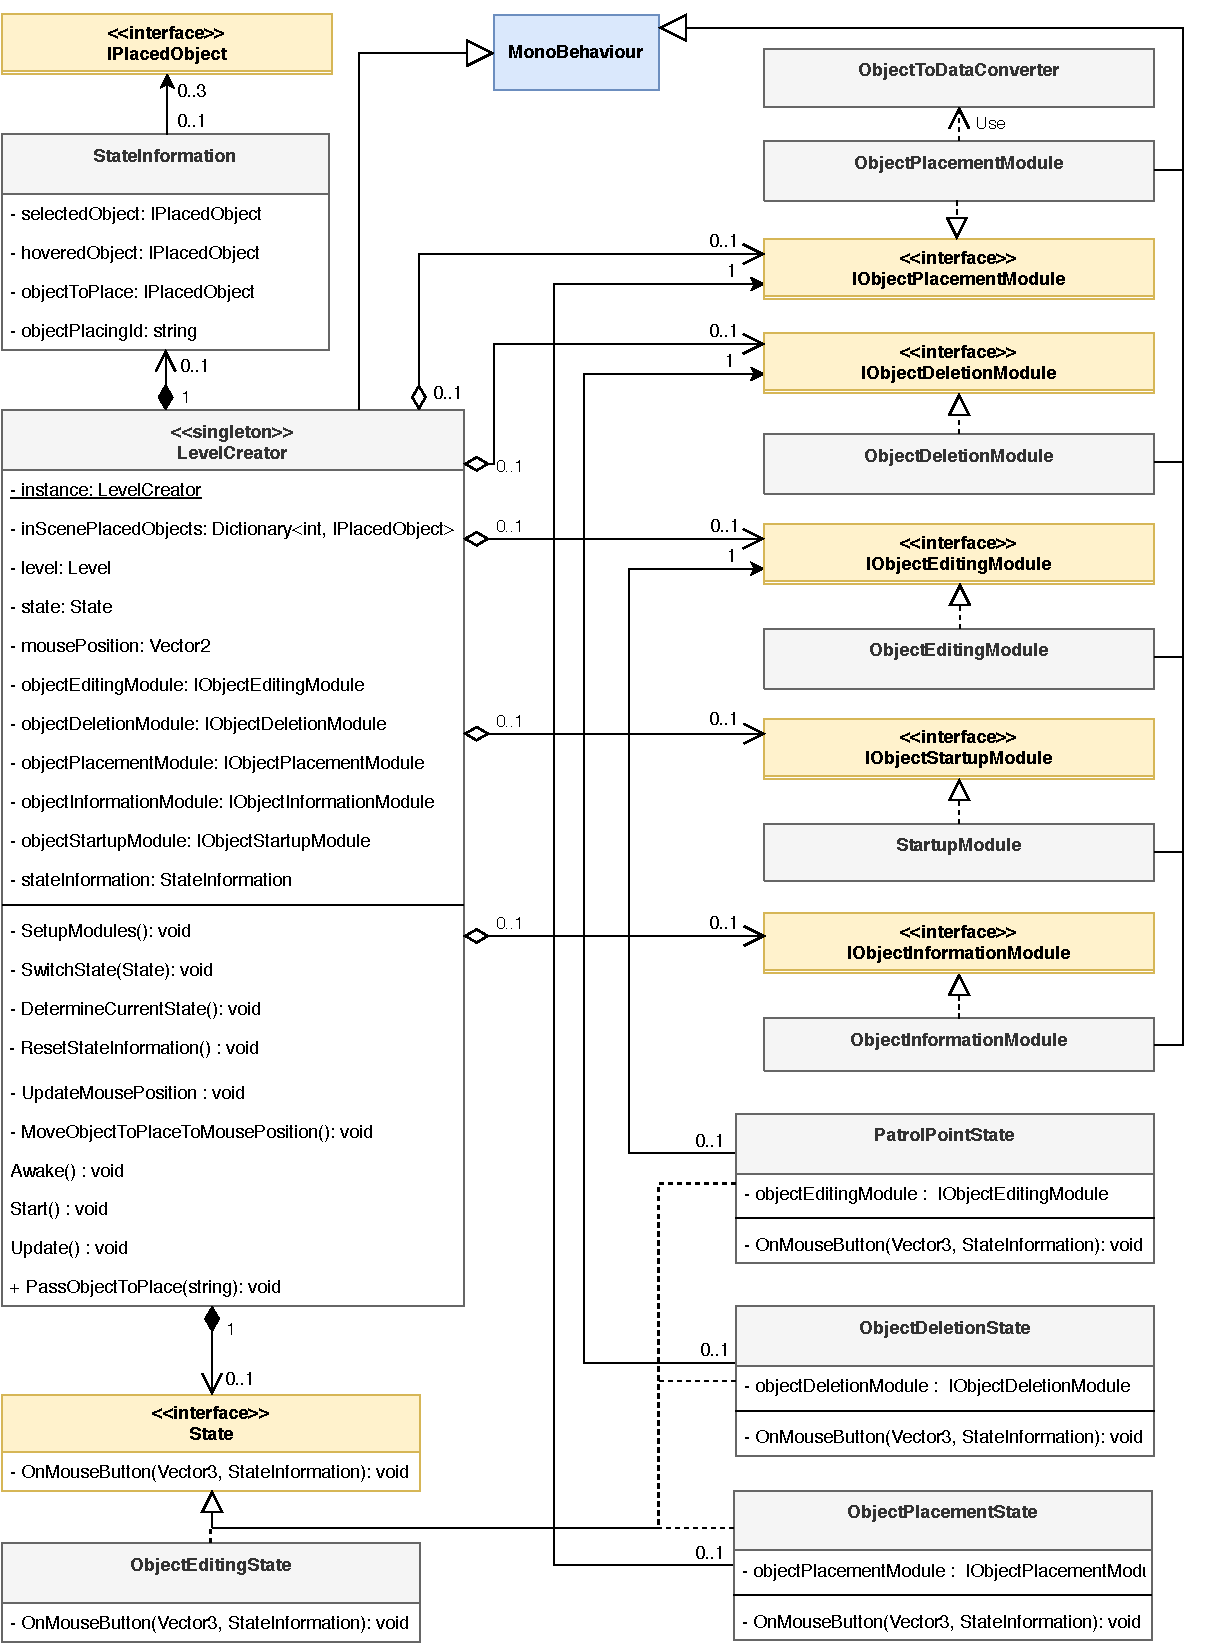
\includegraphics[width=1\textwidth]{pics/leveleditor_levelcreator_compressed.pdf}
		\caption{Der \texttt{LevelCreator}: Die Objektverwaltungskomponente im Level-Editor}
		\label{fig:leveleditor_levelcreator}
	\end {center}
\end {figure}

\subsubsection{Das Platzieren, Löschen und Editieren von 
von Spielobjekten}
Der \texttt{LevelCreator} stellt die Hauptkomponente des Level-Editors dar. Wie bereits erklärt

\begin{itemize}
	\item koordiniert diese Komponente die Initialisierung des Level-Editors und
	\item leitet Informationen an alle anderen Komponenten weiter.
	\item Die Annahme von Ereignissen, Weitergabe von Aufgaben an andere Komponenten und Koordination der Bearbeitung
\end{itemize}

Hierzu hat er selbst folgende wichtige Aufgaben:
\begin{itemize}
	\item Die Bestimmung des aktuellen Zustandes des Level-Editors
	\item Sicherstellung eines \glqq{}sauberen\grqq{} Zustandsüberganges
	\item Aktualisierung und Kontrolle der zu einem Zustand zugehörigen Zustandsinformationen
	\item Weitergabe von Aktionen wie dem Tastendruck der Maus an das aktuelle Zustandsobjekt über die Schnittstelle \texttt{State}
\end{itemize}

Wie bei der Benutzeroberfläche bereits erklärt wurde, gibt es die Zustände Objekterstellung, Objektlöschung, Objektbearbeitung und den Modus für das Setzen der Patroullienroute eines im Bearbeitungsmodus befindlichen Gegners. Ein Tastenklick mit der linken Maustaste kann dabei je nach Zustand eine andere Wirkung haben. Bei der Implementierung wurde daher das als \textit{State-Design-Pattern}\cite{Gamma.2011} bekannte Entwurfsmuster genutzt. Die für das Bearbeiten, Erstellen und Löschen eines Spiels notwendige Funktionalität lässt sich jedoch nur sehr schwer voneinander trennen, da diese Funktionalitäten oftmals voneinander stark abhängen. Beispielsweise werden im Platzierungsmodus alle Waffen und Gegner auf einem Levelstück gelöscht, wenn dort ein Levelelement platziert wird. Auf die zugehörige Funktionalität muss auch im Platzierungsmodus zugegriffen werden können. Um die Abhängigkeiten voneinander so gering wie möglich zu halten und eine Struktur hineinzubringen, wurde die gesamte Funktionalität in insgesamt 5 Module unterteilt und für den Zugriff auf jedes Modul, ein Interface implementiert. Abbildung \ref{fig:leveleditor_levelcreator} zeigt das entstandene Designkonzept für die Implementierung des \texttt{LevelCreators}. Aus Gründen der Übersichtlichkeit und aus Platzmangel mussten alle Methoden in den Modulen und zugehörigen Interfaces, sowie unwichtige Attribute in der Klasse \texttt{LevelCreator} weggelassen werden. 

Die Klasse \texttt{LevelCreator} kontrolliert den Zustand des Levels, während bei Aktionen je nach Zustand unterschiedliche Funktionalitäten vom jeweiligen Zustandsobjekt aufgerufen werden. Aktuell wird das Zustands-Entwurfsmuster nur für einen Tastendruck der linken Maustaste verwendet, dennoch ermöglicht dieses, das Verhalten des Level-Editors schnell anzupassen oder zu erweitern. Wie zu sehen, ist die eigentliche Funktionalität, dargestellt durch die Module, in die Bereiche Erstellen, Informationsausgabe, Editieren, Löschen, und Startup unterteilt. Diese Unterteilung wurde nach dem \textit{CRUD}-Prinzip\cite{Torim.2012} (Create, Read, Update, Delete) gewählt. Wie allgemein bekannt ist, können verschiedene Aktionen meist in die Bereiche Informationsausgabe (Read), Änderung (Update), Löschen (Delete) und Erstellen (Create) eindeutig eingeordnet werden. Der weitere Bereich Startup enthält Funktionalität, die ausschließlich zur Initialisierung eines Levels benötigt wird. Hierzu zählt beispielsweise das Setzen der äußeren Wände zur Randbegrenzung oder die Funktionalität zur Konvertierung der durch den \texttt{LevelController} geladenen Spielobjekte, die im nächsten Abschnitt genauer erläutert wird. 

Mit Hilfe der Methode \texttt{SwitchState()} wird der Zustand gewechselt. Dabei ist es auch möglich von einem Zustand wieder in den gleichen zu wechseln. Wird zum Beispiel im Objektbearbeitungsmodus auf ein anderes Objekt geklickt, so wird dieser Zustand beibehalten und die aktuellen Eigenschaften für das neu ausgewählte Objekt im Objektbearbeitungsbereich der Benutzeroberfläche angezeigt. Wird hingegen im Objektplatzierungsmodus auf die Schaltfläche für das bereits ausgewählte Objekt noch einmal gedrückt, so wird der Platzierungsmodus verlassen  und der Level-Editor befindet sich im Leermodus. Analog tritt dieser Fall ein, wenn im Löschmodus die Schaltfläche zum Aktivieren des Löschmodus gedrückt wird. Wechselt der Editor in den Leermodus, so wird immer die Methode \texttt{ResetStateInformation()} aufgerufen. Hierbei werden die im Zustandsinformations-Objekt gespeicherten Informationen gelöscht. In diesem Objekt werden die aktuell markierten, ausgewählten oder zu platzierenden Objekte, falls vorhanden, gespeichert. Mit Hilfe dieser Informationen kann im Objekt des aktuellen Zustandes die richtige Information entnommen und zur Bearbeitung an die Module weitergegeben werden. Dabei ist wichtig zu wissen, dass immer nur ein Zustand im Level-Editor gleichzeitig aktiv sein kann.
 

\subsubsection{Die Datenverwaltung und das Laden und Speichern eines Levels}
\begin {figure}[h]
	\begin {center}
	    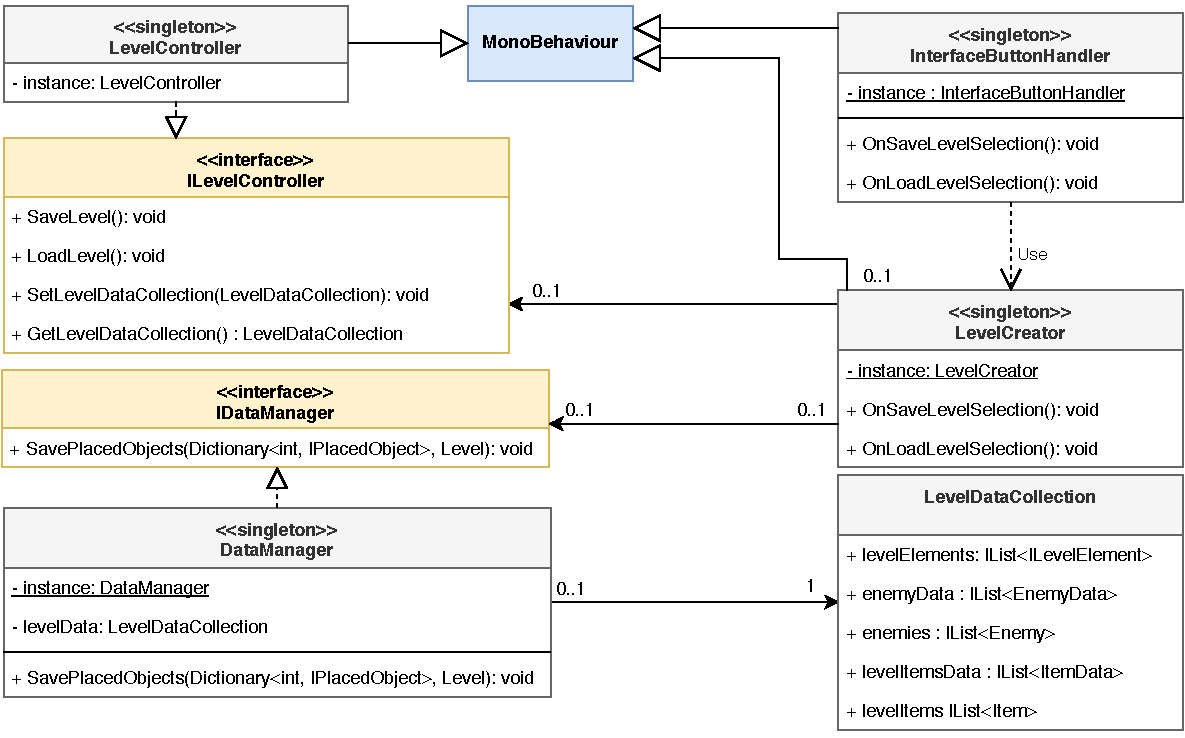
\includegraphics[width=1\textwidth]{pics/leveleditor_levelcontroller.pdf}
		\caption{Das Laden und Speichern mit Hilfe des \texttt{LevelControllers}}
		\label{fig:leveleditor_levelcontroller}
	\end {center}
\end {figure}

Für das Laden eines Levels zum Bearbeiten im Level-Editor oder das Speichern eines Levels im Editor kann bereits auf die Funktionalität zur Serialisierung und Deserialisierung im \texttt{LevelController} zurückgegriffen werden. Mit Hilfe dieser Komponente und der Datenverwaltungskomponente wird das Speichern und Laden eines Levels umgesetzt. Dabei wurde ein Interface eingeführt, um die Abhängigkeiten zwischen dem \texttt{LevelController} und dem \texttt{LevelCreator} so gering wie möglich zu halten.

Die Aufgabe der Datenverwaltung ist es die Daten zu den im Level befindlichen Spielobjekten zu verwalten, damit bei Speicherung des Levels alle für die Serialisierung notwendigen Informationen an den \texttt{LevelController }übergeben werden können. Diese eigenständigen Komponenten werden beim Speichern nacheinander ausgeführt, d.h. es werden die erstellten Informationen über die im Level befindlichen Spielobjekte von der Datenverwaltungskomponente über den \texttt{LevelCreator} an den \texttt{LevelController} über die Schnittstelle \texttt{ILevelController} übergeben. Dabei werden werden die Methoden \texttt{SetLevelDataCollection(...)} zur Aktualisierung der Referenzen auf die Daten und die Methode \texttt{SaveLevel()} aufgerufen, um den \texttt{LevelController} den Befehl zur Serialisierung und somit zur Speicherung des Levels zu geben. 

Für das Laden eines Levels wird zunächst die Methode \texttt{LoadLevel()} der Schnittstelle genutzt, um die Spielobjekte aus den gespeicherten Daten erstellen zu lassen. Nach dem Laden werden die im Objekt \texttt{LevelDataCollection} gespeicherten Referenzen zu diesen Spielobjekten vom \texttt{LevelCreator} über die Methode \texttt{GetLevelDataCollection()} des Interfaces geladen. Um diese Spielobjekte im Level-Editor bearbeiten zu können, ist es notwendig diese in das Format des Level-Editors zu übersetzen. Hierfür muss das \textit{Prefab} jedes Spielobjektes bestimmt und das zugehörige Container-Objekt im \texttt{PrefabsManager} geladen werden. Da die Eigenschaften des Spielobjektes des \textit{Prefabs} aus dem \texttt{PrefabsManager} wie die Position nicht mit den Eigenschaften des geladenen \textit{Prefabs} übereinstimmen, muss das im Container-Objekt untergeordnete Spielobjekt gegen das geladene Spielobjekt ersetzt werden. Danach werden die Position auf das Container-Objekt übertragen, bestimmte Komponenten des Spielobjektes deaktiviert und der \textit{Collider} des jeweiligen Spielobjektes auf das Container-Objekt übertragen.
